\chapter{Funcionalidades Destacadas}


\section{Control de Usuarios}
	É preciso un mínimo control de usuarios para controlar que sube vídeos á plataforma.

\section{Carga de Vídeo}
	Dado que a aplicación traballará con vídeos subidos polos usuarios, o primeiro paso é lograr
	a subida exitosa de vídeos á plataforma. Para este fin empregarase un formulario HTML que 
	viaxa sobre unha chamada POST de HTTP. Cando o navegador faga esta chamada incluíndo o vídeo
	como parte do formulario, este vídeo comezará a subirse ao servidor en pequenos anaquiños 
	(data chunk).
	
	É de especial importancia que no caso de que o vídeo teña un peso considerable e precise 
	duns cantos segundos para subirse á plataforma, o usuario poida coñecer de forma gráfica
	o avance deste proceso.
	
	Con este fin, crease un sistema de notificación de progreso baseado no 
	django-progressbarupload \cite{django-progressbarupload}, este sistema apoiase nunha compoñente
	fundamental chamada VideoUploadHandler, que é unha extensión da interface de Django 
	TemporaryFileUploadHandler \cite{TemporaryFileUploadHandler}, e que basicamente manexa a subida
	dun ficheiro de tamaño considerable.\\
	
	Esta compoñente componse dunha función de inicio (handle\_raw\_input) que crea unha entrada 
	na Cache de Django, almacenando como chave un número aleatorio e a IP do cliente que está a
	subir o vídeo, e como valor o tamaño do ficheiro e o porcentaxe de este que xa está subido.
	Esta entrada será actualizada cada vez que o servidor reciba un novo anaco de vídeo (mediante
	a outra función do compoñente VideoUploadHandler, receive\_data\_chunk). 
	
	Por outra parte, para que visualmente o cliente poida ver o avance da subida a través unha
	barra de progreso, crease unha función asíncrona en javascript (Tecnoloxía AJAX), que 
	periodicamente consulta ao servidor para obter o valor da cache que indica a porcentaxe de
	subida do vídeo, e unha vez obtido, actualiza a barra de progreso para mostralo. Todo isto
	ten lugar no navegador mentres este inda está a subir o arquivo de vídeo.

	Unha vez que a subida se completa, o POST é manexado pola vista UploadView, que se todos
	os datos do formulario son correctos, encargase de crear un modelo VideoModel. Como parte
	desta creación o vídeo pasa do directorio temporal no que foi almacenado (baixo linux por 
	defecto é /tmp) a un directorio calculado pola función get\_valid\_filename. Esta función
	pásaselle ao modelo como parte do seu campo ''video'' do tipo FileField.
	
	\begin{figure}[htp]
	\begin{center}
		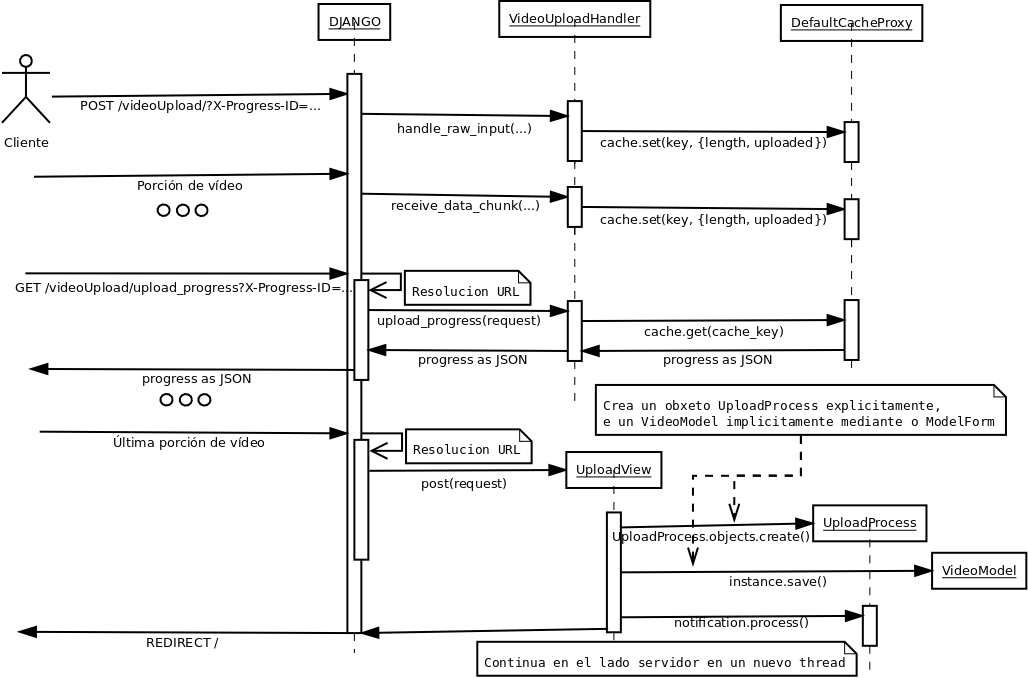
\includegraphics[scale=0.3]{figures/SubidaVideo.png}
		\caption{Diagrama de secuencia do proceso seguido cando se fai o Submit do Formulario 
		de creación de vídeos}
	\label{fig:SubidaVideo}
	\end{center}
	\end{figure}
	
	Unha vez subido o vídeo satisfactoriamente xa está asentada a base da nosa aplicación. Con esta
	parte completada a seguinte funcionalidade a atender será a de mostrar todos os vídeos 
	dispoñibles na plataforma.

\section{Lista de vídeos e Imaxe de Portada}
    Co fin de que os usuarios accedan aos distintos vídeos subidos, deseñase unha páxina web que será a
    principal do módulo video\_manager na cal un usuario pode visualizar unha \textbf{ lista paxinada dos
    vídeos} dispoñibles. Esta lista estará ordenada comezando polo vídeo mais recente e rematando
    polo mais antigo, tamén se contempla a posibilidade de poder filtralos por exemplo polo nome.
    
    Para a elaboración de esta páxina empreganse o elementos dos que dispón Django como son a
    clase ListView co seu atributo paginate\_by e o filtrado de resultado co método 
    QuerySet.filter(...), mentres que para o paso das palabras claves polas que buscar un vídeo
    empregase un parámetro de URL chamado 'name'.\\
    
    Outra funcionalidade interesante de cara a amosar unha lista de vídeos é a de poder mostrar unha
    imaxe representativa de cada un deles. Con este fin crease a vista SuccessfulUpload, á que se
    redirecciona unha vez o vídeo é subido correctamente para seleccionar a súa \textbf{imaxe de portada}.
    
    \begin{figure}[htp]
    \begin{center}
        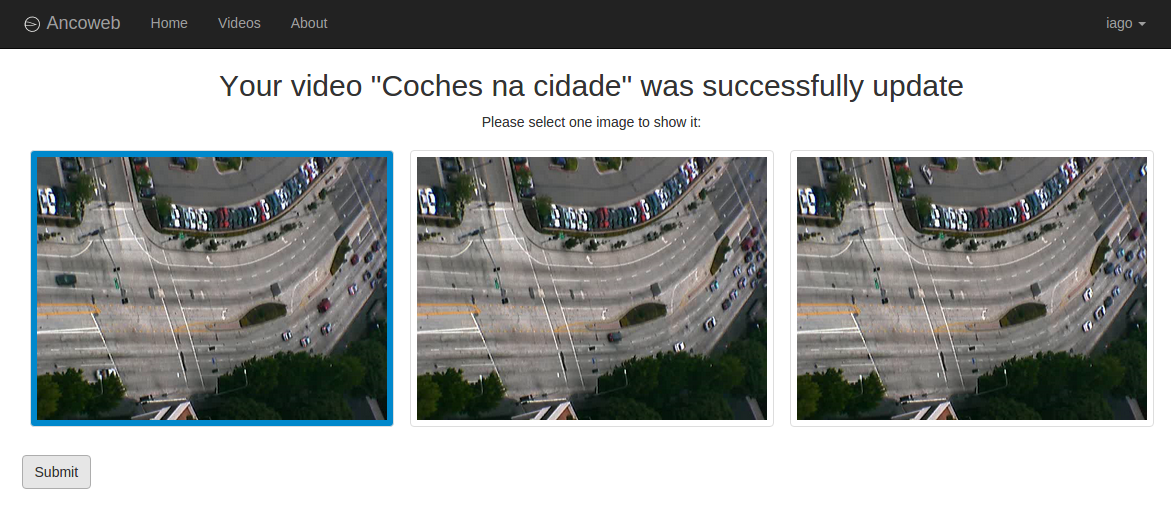
\includegraphics[scale=0.35]{figures/SuccessfulUploadScreen.png}
        \caption{Captura de pantalla da páxina web SuccessfulUpload}
    \label{fig:SuccessfulUploadScreen}
    \end{center}
    \end{figure}
    
    Con este fin extráense mediante ffmpeg unha serie de fotogramas do vídeo, que se gardan nun
    directorio temporal para que unha vez o vídeo estea subido e analizado, as imaxes se integren 
    como parte dun formulario na páxina SuccessfulUpload. Mediante este formulario, xerado co plugin
    image-picker\cite{ImagePickerPage}, o usuario poderá escoller o fotograma que lle pareza mais
    representativo do vídeo e unha vez que pulse no botón de ''Submit'' este fotograma gardarase
    como parte do Modelo de Django VideoModel, quedando pois accesible para que a lista de vídeos 
    poida amosalo.
    
	
\section{Reprodución de Vídeo}
    Desexase que a aplicación permita a reprodución dos vídeos contidos, mediante técnicas de
    streaming ou pseudo-streaming. Neste caso empregarase o pseudo-streaming polo sinxela que
    resulta esta implementación empregando as capacidades da etiqueta $<video>$ de HTML5 en conxunto
    con un servidor HTTP como Apache ou o servidor para desenvolvemento de Django.

    \begin{figure}[htp]
    \begin{center}
        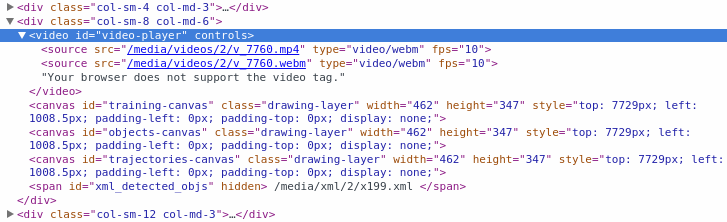
\includegraphics[scale=0.55]{figures/VideoTagHtml5.png}
        \caption{tag en html5, coas súas fontes e coas capas $<canvas>$ asociadas}
    \label{fig:VideoTagHtml5}
    \end{center}
    \end{figure}
    
    na figura \ref{fig:VideoTagHtml5} podemos ver o resultado en HTML5, vense claramente a etiqueta
    $<video>$ coas súas fontes de datos $<source>$, cabe destacar que aquí engadiuse o atributo fps
    (Fotogramas Por Segundo do inglés Frames per second) que non pertence ao estándar definido pola 
    W3C\ref{w3schools-source-tag} mais no caso da nosa aplicación é fundamental para poder coñecer 
    a velocidade á que o navegador vai amosar os fotogramas do vídeo.
    
    Outra cuestión a aclarar é o motivo polo cal non se subministra a fonte de vídeo en formato
    .ogv que a W3C recomenda. A resposta é que o codec theora que ffmpeg inclue soporta 
    decodificación pero NON codificación, polo cal é posible pasar de vídeos en .ogv a outros 
    formatos pero non de outros formatos a .ogv imposibilitando pois que se poida ofrecer o 
    vídeo neste formato mentres o codec de ffmpeg non o permita. Non obstante, isto non supón un 
    problema, xa que como se pode ver na táboa seguinte todos os navegadores permiten a reprodución
    baseándose nestes dous formatos:
    
    % Please add the following required packages to your document preamble:
    % If you use beamer only pass "xcolor=table" option, i.e. \documentclass[xcolor=table]{beamer}
    \begin{table}[]
        \centering
        \caption{My caption}
        \label{my-label}
        \begin{tabular}{llll}
            \rowcolor[HTML]{EFEFEF} 
            Internet Explorer & SI                                                                                              & NON & NON \\
            Chrome            & SI                                                                                              & SI  & SI  \\
            \rowcolor[HTML]{EFEFEF} 
            Firefox           & \begin{tabular}[c]{@{}l@{}}SI \\ dende Firefox 21 (win)\\ dende Firefox 30 (linux)\end{tabular} & SI  & SI  \\
            Safari            & SI                                                                                              & NON & NON \\
            \rowcolor[HTML]{EFEFEF} 
            Opera             & \begin{tabular}[c]{@{}l@{}}SI\\ dende Opera 25\end{tabular}                                     & SI  & SI 
        \end{tabular}
    \end{table}

\section{Análise de Vídeo}
	Para a análise de vídeo será preciso definir unha interface de liña de comandos mediante
	a cal a aplicación web chamará ao Sistema de Recoñecemento, indicándolle aqueles parámetros
	que sexan precisos\ref{fig:InterfazLineaComandos}.

	\subsection{Interface de Liña de Comandos}
	A aplicación web indicaralle a este sistema o vídeo que debe empregar como entrada para o 
	recoñecemento e o ficheiro de saía onde ten que escribir os datos da análise. A maiores, pódeselle
	indicar con que frecuencia se desexa que o Subsistema Behaviour System, encargado da análise de
	alto nivel, entre en funcionamento. Po último a opción --standar fai que se mostre o resultado da
	detección de obxectos por liña de comandos, esta saída é empregada pola capa web para calcular o
	progreso do proceso de análise.\\
	
	Estas opcións tamén se poden visualizar mediante o comando --help:\\ 
	\begin{verbatim}
		iago@UbuIago:~/TFG/src/RecognitionSystem$ ./recognitionsystem --help
		Usage:   recognitionsystem
		option:  
		-i          --input      <path/to/outputFile.xml> Set the input file.
		-o          --output     <path/to/outputFile.xml> Set the output file.
		-f [value]  --frequency  Determines after how many frames the Behaviour 
		                         System checks the minimal path
		--standar                Print the xml into the standar output.
		--verbose
	\end{verbatim}
	
	\begin{figure}[htp]
	\begin{center}
		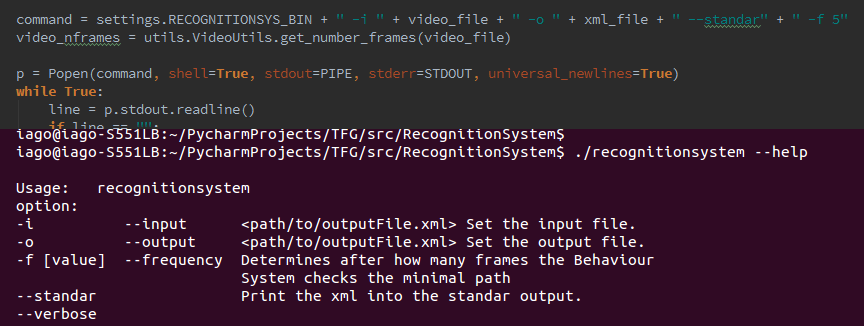
\includegraphics[scale=0.45]{figures/InterfazLineaComandos.png}
		\caption{Interfaze de liña de comandos do Sistema de recoñecemento}
	\label{fig:InterfazLineaComandos}
	\end{center}
	\end{figure}
	
	\subsection{Ficheiro XML}
		Como resultado desta chamada, o sistema de recoñecemento debe crear no ficheiro indicado 
		para a saída, un XML co formato que se define no esquema .dtd situado no directorio
		
		\begin{verbatim}
		src/static/detections\_schema.dtd
		\end{verbatim}		 

		Neste ficheiro podemos ver a definición dos seguintes elementos:
		\begin{itemize}
		\item{{\textbf{$<objects>$\\}}}
			Contén para cada un dos fotogramas $<frame>$ a lista de obxectos detectados segundo
			o explicado no apartado \ref{cap:DeteccionObxetos}, indicando para cada un deles a
			distancia á parte esquerda, e superior da escena (xc, yc) e o alto e ancho do obxecto
			detectado (h, w).
		\item{{\textbf{$<trajectories>$\\}}}
			Este outro elemento garda para cada un dos obxectos detectados a traxectoria que 
			seguiu ao longo do vídeo, esta traxectoria estará composta de unha serie de puntos
			$<point>$, para cada un dos cales, a parte das súas coordenadas e o número de 
			frame, indicase un grao de anormalidade entre 1 e 0 que indica como de anómala é 
			a conduta dese obxecto no momento no que se atopa sobre ese punto.
		\end{itemize}
		
		Para xerar este ficheiro XML foi preciso desenvolver unha serie de funcionalidades en C++,
		que están contidas no paquete XmlRecognition.
	
	\subsection{Paquete XmlRecognition}
		Inicialmente o proxecto conta cun código escrito en C++ e apoiado en OpenCV que está distribuído en
		dúas librerías EllipseLib e BehaviorLib. A primeira delas encargada da detección de obxetos, e a segunda
		encargada de analizalo comportamento a alto nivel a partir dos resultados que proporciona a primeira.\\
		
		Para a construción do Sistema de recoñecemento integraranse estas dúas librerías como módulos, e 
		crearase un terceiro módulo C++ chamado XmlRecognition. Este novo módulo será o responsable de definir e
		implementar a interface de liña de comandos, xestionar a comunicación entre as dúas librerías e gardar
		o resultado da análise en formato XML.\\
		
		Para elo, crease un ficheiro principal chamado \textbf{main.cpp} que describe a interface de liña de comandos
		independente da librería que se emprega para as deteccións, un ficheiro \textbf{XmlUtils} que contén as
		funcionalidades para a escritura do XML en base a unha detección simplificada: DetectionDto 
		(Data Transfer Object), e por último un ficheiro \textbf{RecognitionFacade} que variará en 
		caso de cambiar as librarías, transformando o resultado destas en DetectionDto's para logo
		poder escribilo coas funcionalidades de XmlUtils.
		
		Para maximizar o rendemento evitase crear clases innecesarias: para o caso da DetectionDto é dabondo
		cunha estructura, e no caso de XmlUtils y RecognitionFacade, ao non ter estado chega con ficheiros
		que definen funcións.
		
		\begin{figure}[htp]
		\begin{center}
			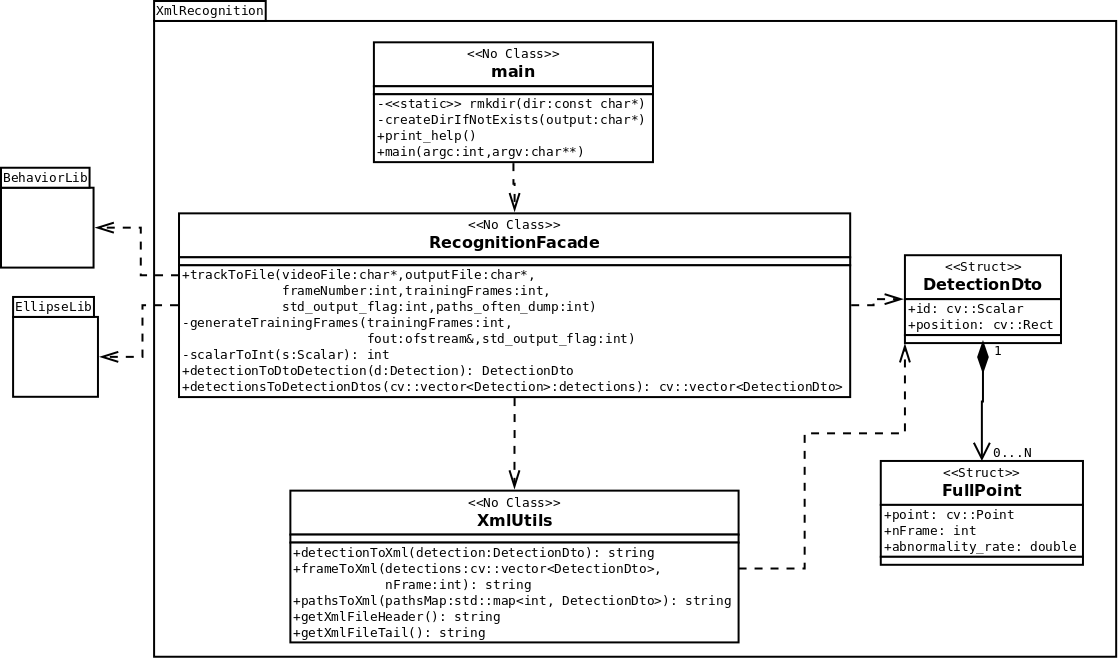
\includegraphics[scale=0.25]{figures/PaqXmlRecognition.png}
			\caption{Diagrama de clases do paquete XmlRecognition}
		\label{fig:PaqXmlRecognition}
		\end{center}
		\end{figure}
		
		Coa elaboración deste paquete queda listo o sistema de recoñecemento, agora solo resta que a capa web
		sexa capaz de chamar ao sistema e mostrar as análises en XML sobre o vídeo. Será o que abordaremos
		no seguinte apartado.
		
	\subsection{A análise dende a capa web}
	
		Cando deseñamos unha aplicación web é de capital importancia que o usuario este informado de que está
		a acontecer na aplicación para que non sinta que está perdido, ou que a aplicación non responde. Tendo
		isto en conta, e sabendo que tanto o proceso de análise coma o de conversión do vídeo a outros 
		formatos poden requirir dun tempo prolongado, prantexase un problema: como manter ao usuario informado
		destes longos procesos e evitar a sensación de bloqueo?\\
		
		A solución deseñada é un sistema de notificacións que permite ao usuario rexistrado navegar libremente
		pola aplicación mentres o vídeo se está a analizar, mostrando en todo momento unha barra de progreso
		para o proceso que se está a seguir nestes intres.
		
		\begin{figure}[htp]
		\begin{center}
			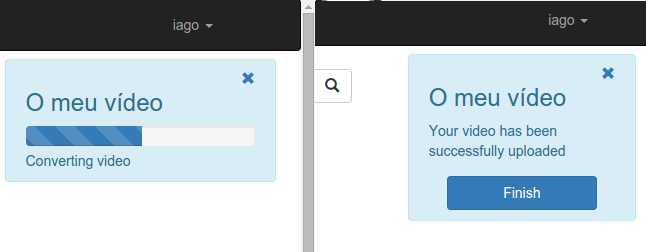
\includegraphics[scale=0.5]{figures/Notificacions.png}
			\caption{Capturas de pantalla do sistema de Notificacións}
		\label{fig:Notificacions}
		\end{center}
		\end{figure}
		
		Para albergar tanto o sistema de notificacións como os procesos que engloba, creouse o módulo de 
		Django video\_upload composto polas clases que se poden observar no seguinte diagrama:

		\begin{figure}[htp]
		\begin{center}
			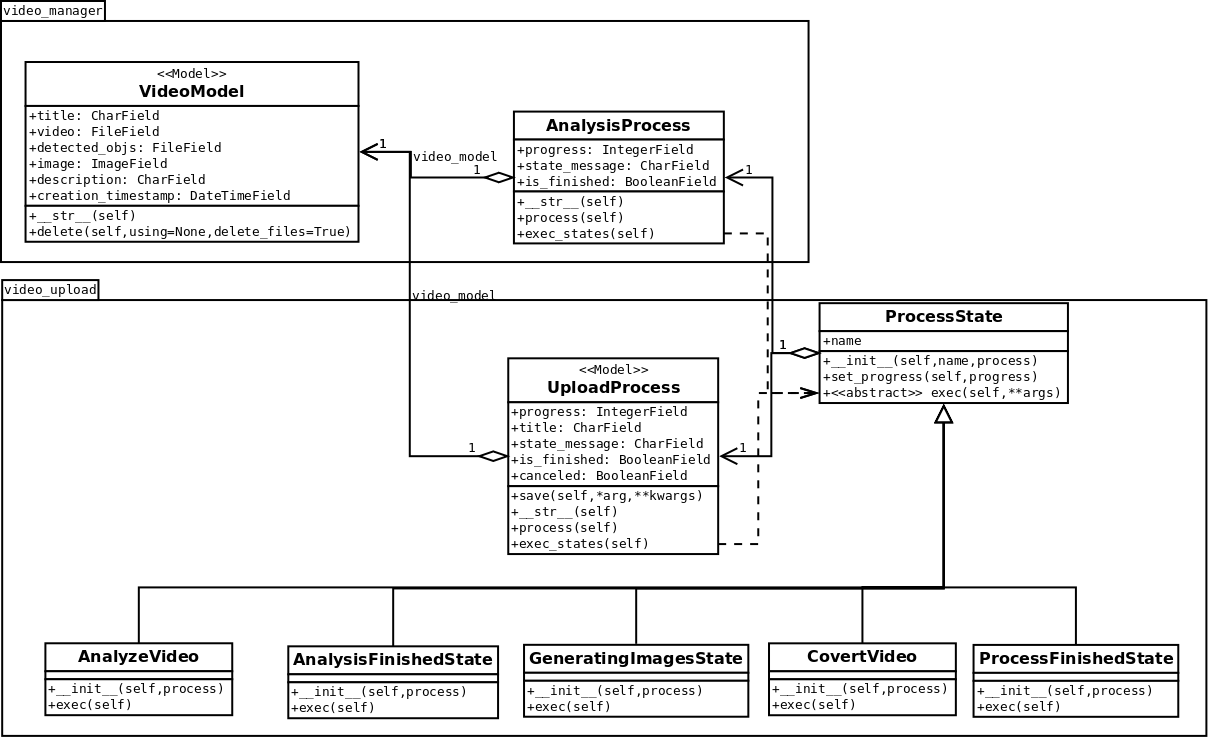
\includegraphics[scale=0.25]{figures/ClassDiagram.png}
			\caption{Diagrama de Clases do sistema}
		\label{fig:ClassDiagram}
		\end{center}
		\end{figure}
		
		UploadProcess representa o proceso de subida, análise, conversión e extracción de imaxes
		a partir de un vídeo. Mentres que AnalysisProcess representa o proceso que se segue no 
		caso de que un vídeo xa subido á plataforma sexa analizado de novo. Os distintos estados
		nos que pode estar un proceso modelanse mediante a clase abstracta ProcessState, que nas
		súas implementacións define tanto o traballo a realizar neste estado coma a mensaxe que 
		se amosará ao usuario cando este se execute.\\
		
		Dado que é o ProcessState que executará a tarefa, tamén será o encargado de actualizar
		a través do método set\_progress(self, progress) o progreso do proceso asociado (
		UploadProcess ou AnalysisProcess).\\
		
		É importante destacar que as figuras etiquetadas co estereotipo $<<Model>>$ son modelos 
		de BD manexados por Django. Nótese tamén que pese a que UploadProcess e AnalysisProcess
		comparten a meirande parte do seu código, non foron refactorizados nunha clase abstracta,
		dadas as complicacións de base de datos que isto carrexa. En lugar diso empregase o 
		tipado dinámico de Python para pasar os obxectos tanto de UploadProcess como de 
		AnalysisProcess á clase ProcessState, que ao invocar só os métodos comúns non é capaz de 
		percibir a diferenza
		entre ambas.
		
		O seu funcionamento mostrase no gráfico:
		
		\begin{figure}[htp]
		\begin{center}
			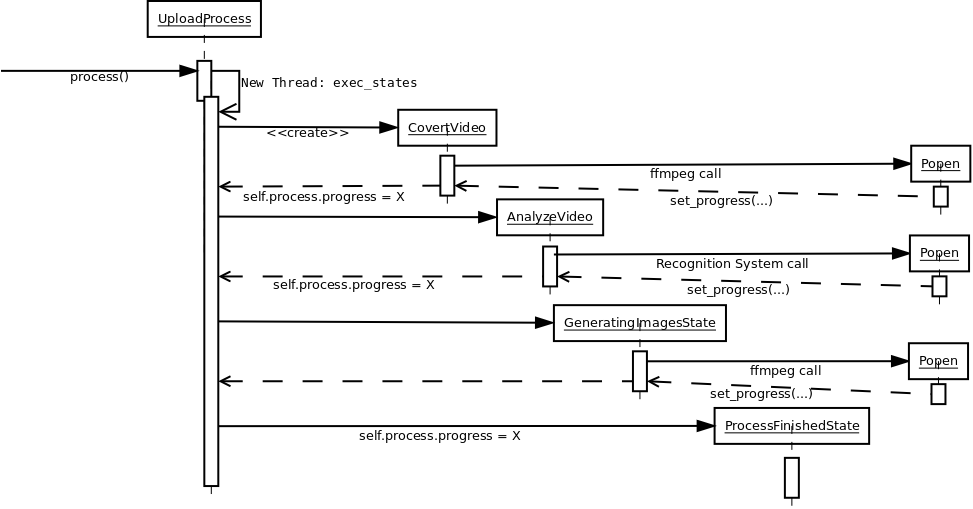
\includegraphics[scale=0.3]{figures/AnaliseVideoWeb.png}
			\caption{Diagrama de secuencia da análise do vídeo na capa web}
		\label{fig:AnaliseVideoWeb}
		\end{center}
		\end{figure}

\section{Mostrar Deteccións}
	
	Unha vez que o vídeo xa está subido e correctamente analizado, o que resta é comezar a construír
	na capa web as vistas que mostren sobre o elemento $<video>$ de HTML5 as distintas capas de 
	análise obtidas a partires do ficheiro XML, así como unha serie de paneis que permitan 
	configurar estas vistas.
	
	Todo este traballo realizase na vista DetailsView do módulo video\_manager e principalmente 
	consiste nun ficheiro HTML que contén as referencias a:
	\begin{itemize}
     \item O vídeo a mostrar
     \item O ficheiro XML que contén a análise realizada polo sistema de recoñecemento.
     \item Os ficheiros de estilo.
     \item Os distintos ficheiros de código javascript involucrados.
    \end{itemize}
    
    
\section{Traxectorias}

\section{Comportamento anormal}
